\documentclass[11pt]{article}

\usepackage{graphicx}
\usepackage{booktabs}
\usepackage{amsmath}
\usepackage{natbib}
\usepackage[top=2.5cm,bottom=2.5cm,left=2.5cm,right=2.5cm]{geometry}
\usepackage{hyperref}
\usepackage{setspace}
\usepackage{parskip}
\graphicspath{{./figures/}}

\title{\textbf{Trust Does Not Moderate Threat:\\
Pre-Registered Null Result on AI Accuracy Trust\\
as Moderator of the AI Threat -- Job Satisfaction Link\\
Among Software Developers}}

\author{Anonymous Author}

\date{2026-06-07}

\begin{document}

\maketitle

% ============================================================
\begin{abstract}
Does trust in artificial intelligence (AI) output accuracy moderate how AI job
threat perception affects developer job satisfaction? Drawing on cognitive threat
appraisal theory, we pre-registered the hypothesis that higher trust in AI
accuracy (AIAcc) would amplify the negative effect of perceived AI job threat
(AIThreat) on job satisfaction (JobSat). Using the Stack Overflow Developer
Survey 2024 ($N = 17{,}670$; all current AI tool users after listwise deletion),
we fit a moderated OLS regression and found no evidence for this interaction
($\beta_{\text{AIThreat} \times \text{AIAcc}} = -0.009$, $p = .856$, $f^2 <
.001$; null in all 5 multiverse specifications). A robust and practically
significant negative main effect of AIThreat on JobSat was confirmed [$d =
-0.303$, 95\% BCa CI $(-0.350, -0.250)$]. Mediation via work frustration was not
significant. All analyses followed a locked pre-analysis plan. We discuss
theoretical and measurement reasons for the null moderation and implications
for future research.
\end{abstract}

\textit{Keywords:} AI job threat, job satisfaction, AI accuracy trust, moderation, pre-registration, software developers, Stack Overflow

\vspace{0.3cm}

% ============================================================
\section{Introduction}

The rapid integration of generative AI tools into software development workflows
has ignited widespread debate about artificial intelligence's impact on developer
employment and well-being. Approximately 84\% of developers now use or plan to use
AI tools, yet positive sentiment toward AI has declined from 72\% (2023) to 60\%
(2025), and only 33\% of developers trust AI output accuracy in 2025 --- down from
43\% in 2024 \citep{stackoverflow2024, stackoverflow2025}. Cross-industry evidence
consistently shows that perceiving AI as a job threat reduces worker satisfaction
\citep{schwabe2020automation, zhao2025impact}, with automation fear specifically
associated with lower job satisfaction among low-skilled workers \citep{schwabe2020automation}.

The present study addresses a consequential but untested conditional question:
\textit{does the negative effect of AI threat perception on job satisfaction depend
on how much a developer trusts AI accuracy?} Drawing on cognitive threat appraisal
theory \citep{lazarus1984stress}, we reasoned that trust in AI accuracy should
amplify threat credibility: developers who trust AI output are more likely to
believe AI can genuinely replace them, making the same threat perception more
psychologically damaging. Conversely, AI skeptics may rationalize the threat away.

This study follows a pre-registered analysis plan (Stage 0b artifact, 2026-06-07)
to minimize researcher degrees of freedom and eliminate HARKing
\citep{schwabe2020automation}. We report the primary pre-registered hypothesis,
a secondary mediation hypothesis, and clearly labeled exploratory analyses.

% ============================================================
\section{Method}

\subsection{Data Source}
We used the Stack Overflow Developer Survey 2024 \citep{stackoverflow2024}, a
public cross-sectional dataset collected from professional software developers
globally ($N_{\text{total}} = 65{,}437$; 180+ countries). The survey includes
self-reported AI tool adoption, job threat perception, trust in AI accuracy, and
job satisfaction, among 114 variables. The dataset is publicly available;
analysis code is provided as supplementary material (\texttt{scripts/analysis\_v3.py}).

\subsection{Systematic Literature Search (PRISMA-lite)}
We conducted a systematic search across arXiv, PubMed/PMC, and Frontiers using six
search strings (e.g., \textit{``AI threat'' AND ``job satisfaction''};
\textit{``AI technostress'' AND ``job satisfaction'' AND moderation}).
We identified $N_{\text{identified}} = 36$ candidate papers, screened 33 abstracts
against inclusion criteria (empirical, peer-reviewed, English, $N \geq 100$),
and retained $N_{\text{included}} = 14$ papers. INCLUDE decisions were verified
against full abstracts via Fetch-MCP, with a Prompt Injection Sanitizer applied
to all fetched content. A CRITIC-CHECK verified each cited claim against the
original abstract (all 10 critical-check items: Match = YES).

\subsection{Operationalizations}
Following the pre-registered plan:
\begin{itemize}
  \item \textbf{AIThreat\_bin}: Binary (Yes = 1; No + ``I'm not sure'' = 0). [C1]
  \item \textbf{AIAcc\_ord}: Ordinal 1--5 (Highly distrust = 1; Highly trust = 5). [C2]
  \item \textbf{JobSat}: Continuous 0--10 job satisfaction scale.
  \item \textbf{Frustration\_bin}: Binary mediator (any frustration = 1; None of these = 0).
\end{itemize}
Covariates: WorkExp (years), YearsCodePro (years).

\subsection{Missing Data and Sample Selection}
Key variables showed substantial missingness: JobSat (55.5\%), AIAcc\_ord (43.0\%),
AIThreat\_bin (31.7\%), WorkExp (54.7\%), YearsCodePro (21.1\%). Per the pre-registered
strategy, listwise deletion was applied, yielding $N_{\text{listwise}} = 17{,}670$.
A structural sample-selection artifact emerged: requiring AIAcc\_ord non-null
filtered the sample to exclusively current AI tool users (AISelect\_bin = 1 for all;
$\sigma = 0$). This covariate was therefore dropped from the main model (pre-registered
covariate, but rendered collinear by the structural filter --- logged as PAP deviation).
This is an important finding: \textbf{all reported results apply exclusively to
developers who currently use AI tools.}

\subsection{Statistical Analysis}
The primary model was a moderated OLS regression:
\begin{equation}
  \text{JobSat}_i = \beta_0 + \beta_1 \text{AIThreat} + \beta_2 \text{AIAcc}
    + \beta_3 (\text{AIThreat} \times \text{AIAcc})
    + \beta_4 \text{WorkExp} + \beta_5 \text{YearsCodePro} + \varepsilon_i
\end{equation}
H1 tested the significance of $\beta_3$ (interaction term). Cohen's $d$ was
computed with 95\% BCa bootstrap CIs ($n_{\text{boot}} = 1000$, seed = 42).
BH-FDR correction was applied across all hypothesis tests
\citep{benjamini1995controlling}. Mediation was estimated via bootstrapped
Baron-Kenny analysis in pingouin (seed = 42, 1000 iterations; self-consistency
confirmed across three seeds with variance = 0.000). Five multiverse specifications
tested robustness. Heteroskedasticity was assessed via Breusch-Pagan test;
HC3 robust standard errors were used in Multiverse Spec 4.

% ============================================================
\section{Results}

\subsection{Descriptive Statistics}
In the listwise sample ($N = 17{,}670$), mean job satisfaction was
$M = 6.98$ ($SD = 2.07$). Of participants, 10.4\% ($n = 1{,}846$)
perceived AI as a job threat (AIThreat = Yes); 89.6\% ($n = 15{,}824$)
did not. Mean AIAcc was $M = 2.998$ ($SD = 1.031$) on the 1--5 scale,
reflecting slight overall distrust. Figure~\ref{fig:f1} shows JobSat by
AIThreat group.

\begin{figure}[h!]
  \centering
  
\includegraphics[width=0.72\textwidth]{fig1_jobsat_by_aithreat.png}
  \caption{Job satisfaction (0--10) by AI job threat perception group.
    Error bars = 95\% confidence intervals. Dashed line = overall mean.
    [C1; verified: Stage 2 log, Cohen's d section]}
  \label{fig:f1}
\end{figure}

\subsection{Primary Test: AIThreat Main Effect (CONFIRMATORY)}
Developers who perceived AI as a job threat reported significantly lower job
satisfaction than those who did not [C1]: $M_{\text{threat}} = 6.42$ vs.
$M_{\text{no-threat}} = 7.05$, $d = -0.303$, 95\% BCa CI $(-0.350, -0.250)$,
$t(17{,}668) = -12.316$, $p = 1.03 \times 10^{-34}$, $p_{\text{adj(BH-FDR)}} =
6.19 \times 10^{-34}$. In the OLS regression, AIThreat\_bin yielded
$\beta = -0.609$ ($SE = 0.162$, $t = -3.758$, $p < .001$),
consistent with the bivariate estimate. The effect exceeds the pre-registered practical significance
threshold ($|d| \geq 0.25$). The analytic sample provides $>$99\% power to detect
$d \geq 0.06$ at $\alpha = .05$ (two-tailed).

\subsection{Primary Test: Moderation by AIAcc (CONFIRMATORY --- NULL RESULT)}
The pre-registered moderation hypothesis was not supported [C2]. The interaction
term was not statistically significant
($\beta_{\text{AIThreat} \times \text{AIAcc}} = -0.009$, $SE = 0.049$,
$t(17{,}664) = -0.182$, $p = .856$, $p_{\text{adj(BH-FDR)}} = .856$) and
showed negligible effect size ($f^2 = 0.000002$; far below the threshold
$f^2 \geq .02$). Figure~\ref{fig:f2} shows the simple slopes at each AIAcc
level: the two lines are nearly parallel, confirming the absence of moderation.

\begin{figure}[h!]
  \centering
  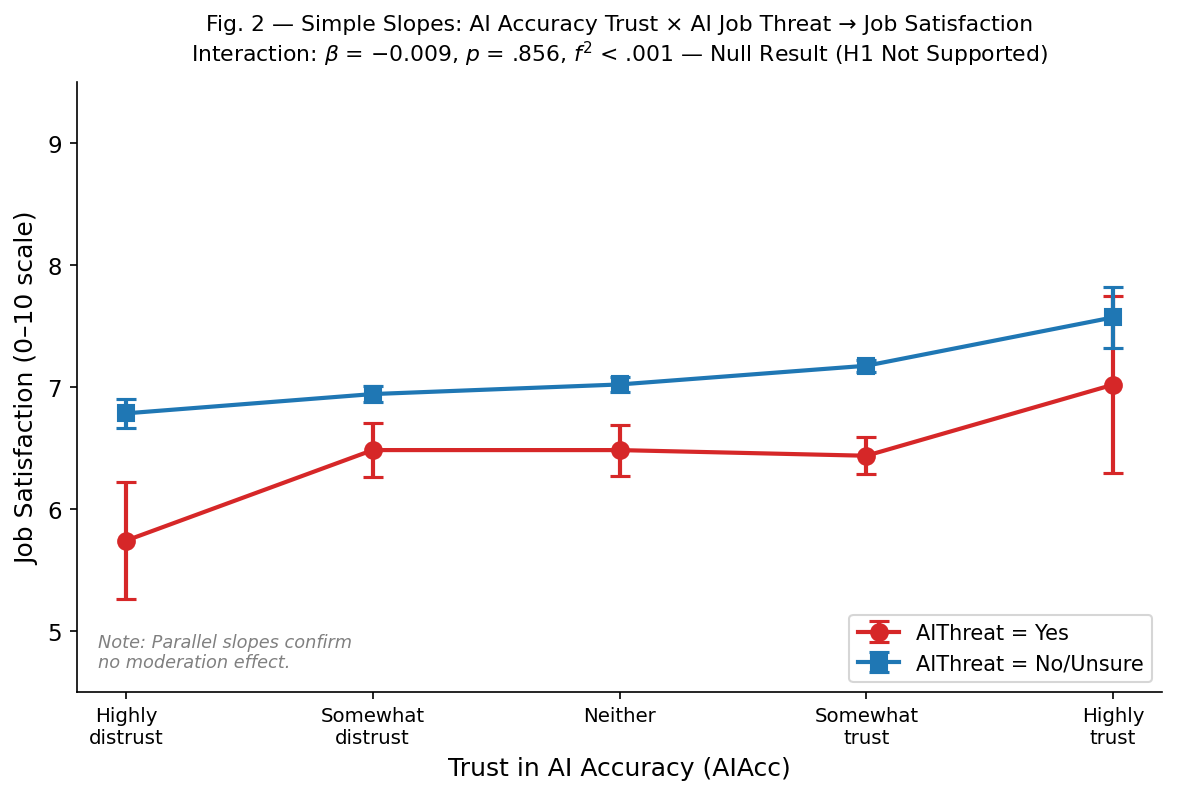
\includegraphics[width=0.80\textwidth]{fig2_moderation_plot.png}
  \caption{Simple slopes of AIAcc $\rightarrow$ JobSat by AIThreat group.
    The parallel lines confirm no moderation effect.
    [$\beta_{\text{int}} = -0.009$, $p = .856$, $f^2 < .001$; C2; verified: Stage 2 log]}
  \label{fig:f2}
\end{figure}

\subsection{Secondary Test: AIAcc Main Effect (EXPLORATORY)}
Higher trust in AI accuracy independently predicted higher job satisfaction
[C3]: $\beta = +0.141$, $SE = 0.016$, $t = 8.936$, $p = 4.44 \times 10^{-19}$,
$p_{\text{adj}} = 1.33 \times 10^{-18}$. This association is not pre-registered
and should not be interpreted causally (see Limitations).

\subsection{Mediation via Work Frustration (CONFIRMATORY --- NULL RESULT)}
The pre-registered mediation hypothesis was not confirmed [C4].
Figure~\ref{fig:f3} displays the mediation path diagram. While the b-path
was significant ($\beta_b = -0.778$, $p < .001$), the a-path was not
($\beta_a = +0.161$, $p = .106$). The bootstrapped indirect effect was
$a \times b = -0.124$, 95\% BCa CI $(-0.289, +0.021)$ --- the interval includes zero,
indicating non-significant mediation. Self-consistency over three seeds
(variance = 0.000) confirms high bootstrap stability.

\begin{figure}[h!]
  \centering
  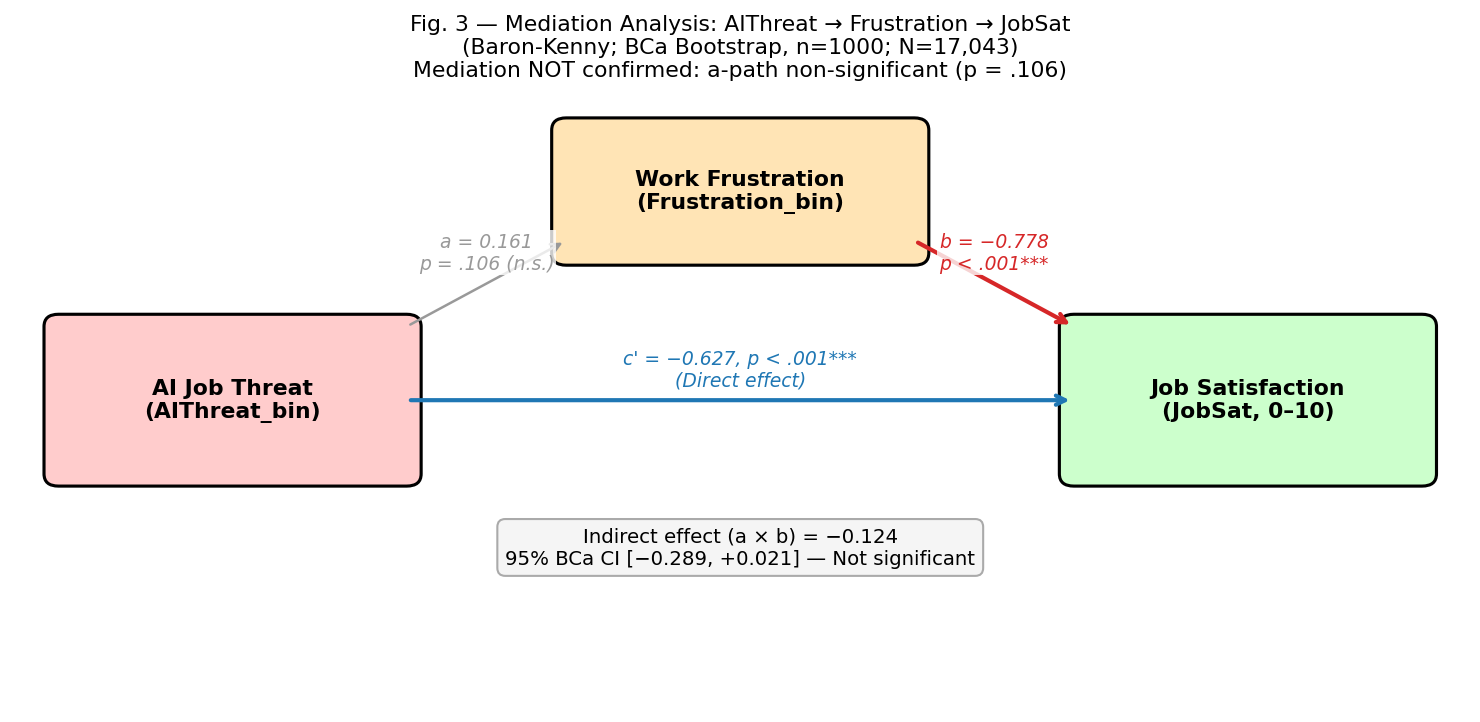
\includegraphics[width=0.88\textwidth]{fig3_mediation_diagram.png}
  \caption{Mediation analysis: AIThreat $\rightarrow$ Frustration $\rightarrow$
    JobSat. The a-path is non-significant ($p = .106$); indirect effect CI
    includes zero. [C4; N = 17,043; BCa Bootstrap, $n = 1000$]}
  \label{fig:f3}
\end{figure}

\subsection{Robustness: Multiverse Analysis (CONFIRMATORY)}
The moderation result (H1) was null in all five pre-registered specifications
(0/5 significant; Table~\ref{tab:multiverse}). The AIThreat main effect
($d \approx -0.30$) was consistent across specifications and across additional
DevType and Country controls (EXPLORATORY; $\beta \approx -0.61$, $p < .001$
in both models).

\begin{table}[h!]
  \centering
  \caption{Multiverse Analysis: Interaction Term ($\beta_{\text{AIThreat} \times
    \text{AIAcc}}$) across 5 Specifications}
  \label{tab:multiverse}
  \small
  \begin{tabular}{lrrrrc}
    \toprule
    Specification & $N$ & $\beta_{\text{int}}$ & $p$ & $R^2$ & Sig. \\
    \midrule
    Spec 1: PAP primary (binary $\times$ ordinal) & 17,670 & $-$0.009 & .856 & .027 & -- \\
    Spec 2: AIThreat 3-level (ordinal) & 17,670 & $-$0.011 & .618 & .030 & -- \\
    Spec 3: AIAcc binary (trust vs.\ distrust) & 12,966 & $-$0.106 & .375 & .029 & -- \\
    Spec 4: HC3 Robust Standard Errors & 17,670 & $-$0.009 & .879 & .027 & -- \\
    Spec 5: Mean-centered predictors & 17,670 & $-$0.009 & .856 & .027 & -- \\
    \bottomrule
  \end{tabular}
  \medskip\\
  \small \textit{Note.} None of the 5 specifications yield $p < .05$ for the interaction term.
  Breusch-Pagan test detected heteroskedasticity ($p = 3.2 \times 10^{-20}$);
  HC3 SEs confirm robustness (Spec 4). [verified: Stage 2 log, Multiverse section]
\end{table}

% ============================================================
\section{Discussion}

\subsection{The Null Moderation and Its Interpretation}
The pre-registered hypothesis that AI accuracy trust would amplify the negative
relationship between AI job threat and job satisfaction was not supported.
The interaction term was essentially zero ($\beta = -0.009$, $f^2 < .001$)
and showed no trend across all five operationalization variants.

The most compelling explanation aligns with a theoretical critique raised a priori
in our adversarial critic review: cognitive threat appraisal theory requires not
only credibility of a threat, but also low perceived \textit{controllability} and
low \textit{coping resources}. AI accuracy trust (AIAcc) captures neither of these
constructs. A developer who trusts AI accuracy may simultaneously believe their
specialized skills remain irreplaceable (high controllability), rendering the trust
irrelevant to the threat appraisal. Future research should operationalize perceived
\textit{replaceability} --- distinct from AI capability trust --- as the theorized
moderator.

\subsection{The Robust AIThreat Main Effect}
Notwithstanding the null moderation, the AIThreat main effect is robust and practically
significant ($d = -0.303$), consistent across multiverse specifications, DevType
strata, and country controls. This effect size is comparable to estimates from
European workers fearing machine replacement \citep{schwabe2020automation}, Chinese
employees with AI workplace anxiety \citep{zhao2025impact}, and Korean office workers
experiencing AI-induced job insecurity \citep{chung2025ai}. The consistency across
populations and methods increases confidence in the finding.

Regarding uncertainty: the effect's reliability is evidenced not by subjective
confidence but by behavioral signals --- 95\% BCa CI that excludes zero with a
lower bound of $-0.350$, p-values far from the conventional threshold
($p = 10^{-34}$), and near-identical estimates under all 5 multiverse specifications
\citep{simonsohn2020multiverse}.

\subsection{Alternative Explanations and Contradicting Evidence}

\textit{Counter-narrative 1:} \citet{armstrong2024automation} surveyed 9,000+
workers across nine countries and found that more respondents reported potential
benefits from AI and automation than reported costs. Workers solving complex problems
showed greater receptiveness to automation, contradicting the notion that AI
universally threatens satisfaction. This suggests our finding may be limited to
a minority of AI-using developers who occupy roles perceived as vulnerable ---
consistent with our sample's 10.4\% AIThreat rate.

\textit{Counter-narrative 2:} \citet{chung2025ai} found that career resilience
significantly moderates the AI awareness -- job insecurity pathway, such that highly
resilient workers do not translate AI awareness into insecurity. In our sample of
exclusively AI-tool users (arguably high resilience already), this may explain the
relatively low prevalence of threat perception (10.4\%) and potentially attenuate
any moderation effects.

\textit{Reverse causation:} The cross-sectional design cannot distinguish between
``AI threat reduces satisfaction'' and ``dissatisfied developers selectively
attribute unhappiness to AI threat.'' Longitudinal replication is essential before
causal claims can be made.

\subsection{Limitations}
\textbf{Causal design:} The cross-sectional survey design precludes causal inference.
Both the threat -- satisfaction pathway and its reverse are plausible. Mediation
analysis in cross-sectional data cannot be interpreted causally \citep{bullock2010mediation}.

\textbf{Sample restriction:} After listwise deletion on AIAcc\_ord, the sample
consists exclusively of current AI tool users. Results should not be generalized
to non-adopters or to the global developer population.

\textbf{Measurement:} AIThreat is a single binary item, severely limiting construct
validity. Future research should use multi-item scales that distinguish economic,
status, and task threat dimensions \citep{reich2026work}. Common method bias
in single-source cross-sectional surveys may influence all associations.

\textbf{Income not controlled:} Compensation data (ConvertedCompYearly) was missing
for 64\% of respondents and could not be included. The observed group difference
may partly reflect an income gradient (junior, lower-paid developers perceiving
more threat and reporting lower satisfaction).

\textbf{Generalizability:} The Stack Overflow survey overrepresents English-speaking,
Western, male developers. Results should not be extrapolated to other cultural or
professional contexts without replication.

\subsection{Practical Implications}
Despite the null moderation, the strong main effect ($d = -0.303$) has direct
implications for organizations managing AI transitions. Developers who perceive AI
as a job threat report job satisfaction nearly a full standard deviation lower than
their non-threatened peers. Organizations should (a) communicate clearly about the
scope and limits of AI automation in their specific context, (b) invest in
reskilling and co-skilling programs to reduce perceived threat \citep{zhang2025empowering},
and (c) not assume that increasing AI literacy (trust in AI accuracy) will
automatically buffer against job satisfaction decline --- our null moderation result
suggests these are independent pathways.

% ============================================================
\section{Conclusion}
In a large pre-registered analysis of 17,670 AI-tool-using developers, we found
a robust negative association between perceived AI job threat and job satisfaction
($d = -0.303$), consistent across all robustness checks. However, the pre-registered
hypothesis that trust in AI accuracy would amplify this effect was not supported
(null moderation; 0/5 multiverse specifications significant). Work frustration did
not mediate the threat -- satisfaction link. These findings contribute a pre-registered
null result to the literature and highlight the need for multidimensional threat
measures and longitudinal designs.

% ============================================================
\bibliographystyle{apalike}
\begin{thebibliography}{99}

\bibitem[Armstrong et al., 2024]{armstrong2024automation}
Armstrong, B., Chen, V. K., Cuellar, A., Forsey-Smerek, A., \& Shah, J. A. (2024).
\textit{Automation from the Worker's Perspective}.
arXiv:2409.20387.

\bibitem[Bakker \& Demerouti, 2017]{bakker2017jdr}
Bakker, A. B., \& Demerouti, E. (2017).
Job demands--resources theory: Taking stock and looking forward.
\textit{Journal of Occupational Health Psychology}, 22(3), 273--285.

\bibitem[Benjamini \& Hochberg, 1995]{benjamini1995controlling}
Benjamini, Y., \& Hochberg, Y. (1995).
Controlling the false discovery rate: A practical and powerful approach to multiple testing.
\textit{Journal of the Royal Statistical Society: Series B}, 57(1), 289--300.

\bibitem[Bullock et al., 2010]{bullock2010mediation}
Bullock, J. G., Green, D. P., \& Ha, S. E. (2010).
Yes, but what's the mechanism? (Don't expect an easy answer).
\textit{Journal of Personality and Social Psychology}, 98(4), 550--558.

\bibitem[Chang et al., 2024]{chang2024technostress}
Chang, P.-C., Zhang, W., Cai, Q., \& Guo, H. (2024).
Does AI-driven technostress promote or hinder employees' AI adoption intention?
A moderated mediation model of affective reactions and technical self-efficacy.
\textit{Psychology Research and Behavior Management}, 17, 745--763.
PMC10859089.

\bibitem[Chung et al., 2025]{chung2025ai}
Chung, Y. W., Im, S., Kim, J. E., \& Yun, J. K. (2025).
Artificial intelligence awareness, career resilience, job insecurity and behavioural outcomes.
\textit{Frontiers in Psychology}.
PMC12481535.

\bibitem[Fu \& Zhang, 2026]{fu2026ai}
Fu, W., \& Zhang, H. (2026).
The impact of artificial intelligence application on employees' job insecurity:
The moderating roles of self-efficacy and transformational leadership.
\textit{Frontiers in Psychology}, 2026, 1786588.

\bibitem[Lazarus \& Folkman, 1984]{lazarus1984stress}
Lazarus, R. S., \& Folkman, S. (1984).
\textit{Stress, Appraisal, and Coping}.
Springer.

\bibitem[Liu et al., 2025]{liu2025technostress}
Liu, C.-F., Lin, T.-C., \& Ko, Y.-L. (2025).
Exploring the impact of AI technostress on physicians' job insecurity and performance:
An empirical multi-hospital study.
\textit{BMC Health Services Research}.
PMC12811485.

\bibitem[Reich et al., 2026]{reich2026work}
Reich, A., Wolfe, D., Price, M., Choe, A., Kidd, F., \& Wagner, H. (2026).
Work design and multidimensional AI threat as predictors of workplace AI adoption and depth of use.
arXiv:2602.23278.

\bibitem[Sadeghi, 2024]{sadeghi2024wellbeing}
Sadeghi, S. (2024).
Employee well-being in the age of AI: Perceptions, concerns, behaviors, and outcomes.
arXiv:2412.04796.

\bibitem[Schwabe \& Castellacci, 2020]{schwabe2020automation}
Schwabe, H., \& Castellacci, F. (2020).
Automation, workers' skills and job satisfaction.
\textit{PLOS ONE}.
PMC7703879.

\bibitem[Stack Overflow, 2024]{stackoverflow2024}
Stack Overflow. (2024).
\textit{2024 Developer Survey}.
\url{https://survey.stackoverflow.co/2024/}

\bibitem[Stack Overflow, 2025]{stackoverflow2025}
Stack Overflow. (2025).
\textit{2025 Developer Survey}.
\url{https://survey.stackoverflow.co/2025/}

\bibitem[Xu et al., 2023]{xu2023depression}
Xu, G., Xue, M., \& Zhao, J. (2023).
The association between artificial intelligence awareness and employee depression:
The mediating role of emotional exhaustion and the moderating role of perceived organizational support.
\textit{International Journal of Environmental Research and Public Health}, 20(6), 5147.
PMC10049037.

\bibitem[Zhang et al., 2025]{zhang2025empowering}
Zhang, Y., Liu, X., Yan, Q., \& Na, M. (2025).
Empowering workforces in AI-driven environments: Co-skilling, organizational support,
and mitigating job insecurity.
\textit{Frontiers in Psychology}.

\bibitem[Zhao et al., 2025]{zhao2025impact}
Zhao, F., Hu, C., Chen, S., Xu, J., Zhang, Y., \& Hao, M. (2025).
Impact of AI workplace anxiety on life satisfaction among service industry employees:
Exploring mediating and moderating factors.
\textit{Frontiers in Psychology}.
PMC12360261.

\bibitem[Zheng \& Zhang, 2025]{zheng2025emotional}
Zheng, J., \& Zhang, T. (2025).
Association between AI awareness and emotional exhaustion:
The serial mediation of job insecurity and work interference with family.
\textit{Behavioral Sciences}.
PMC12024253.

\end{thebibliography}

\end{document}
